\section{Ankneipe SS 2024: Die Oelympischen Spiele}
\sectionmark{Vandalix bei den Oelympischen Spielen}

%\begin{figurehere}
%	\begin{center}
%		\includegraphics[width=\linewidth]{Bilder/andechs2.jpg}
%%		\caption{xxx} 
%	\end{center}
%\end{figurehere}



\begin{multicols}{2}

	20 Uhr. Langsam füllt sich der Kneipsaal. In einer viertel Stunde soll es losgehen. Plätze werden gesucht und reserviert, die ersten Krüge schon wieder nachgefüllt. 
Es werden noch mal ein paar Schlücke in geselliger Runde getrunken, bevor sich alle auch schon an ihre Zapfen begeben. Diese sind gut mit Bundes- und Cartellbrüdern gefüllt. 
Dann ist es so weit: Die Corona erhebt sich, die Hochchargen des Sommersemesters werden angekündigt und der Biermusikus greift voll in die Tasten für den ersten Marsch des Abends.
Gläser klirren. Von überall hört man „Prost!“. Die Würdenträger und Gäste des Abends werden begrüßt und der hohe Senior Benjamin Buhl führt kurz durch das Semesterprogramm. In seiner Rede zur Abkneipe des Wintersemesters erläuterte er uns bereits seine Gedanken zu dem Semesterwahlspruch: „Die Grenzen meiner Sprache bedeuten die Grenzen meiner Welt“. Nun führt er dieses Thema noch weiter aus. Sprache, als die Menschen miteinander verbindendes Element. Sprache, durch die man selbst erst den eigenen Horizont erweitern kann. Darunter fasst er aber nicht nur das Kennenlernen neuer Kulturen – nein, auch das Verbindungsstudententum selbst. Unser Grundprinzip Sciencia verpflichtet uns mit offenen Augen durchs Leben zu gehen und auch abseits der eigenen Fachrichtung den einen oder anderen Wissensfetzen aufzuschnappen. Wissen, welches uns davor bewahren soll auf sogenannte Fake News hereinzufallen. Wissen, das uns aber auch im Diskurs untereinander voranbringen kann. Die Rede endet mit der Ermutigung, immer neugierig, interessiert und im Austausch zu bleiben. Das folgende Kolloquium bildet die perfekte Grundlage für einen solchen Austausch.
Ein Lied nach dem anderen wird gesungen, ein Bier nach dem anderen getrunken.
Dann wird auch schon der Salamander gerieben und aus der Corona erschallt es kollektiv: „Fux, Stoff!“
Nach dem das letzte Lied des hochoffiziellen Teils verklungen ist und sich jeder, der Fuxia sei Dank, mit Leberkassemmeln für den zweiten Teil des Abends stärken konnte, geht es schon weiter.
Bundesbruder Fabian Heinrich schlägt den inoffiziellen Teil des Abends und stimmt uns mit einer kurzen Rede auf das Motto der heutigen Kneipspiele ein. Mental reisen wir ins antike Griechenland. Heute wird Trinksport betrieben - auf o(e)lympischem Niveau. Vor allem beschäftigen wir uns heute mit einer Disziplin: Dem Marathon. Eine Kneipe ist schließlich kein Sprint. Wir befinden uns mittlerweile im zweiten Drittel und steuern auf das Dritte zu, den Ausklang. Nach diversen Bieren und guten Gesprächen neigt sich der Abend dem Ende zu. Der Marathon wurde bezwungen. Gefühlt wurden 42,195 Bierchen getrunken. 
Wohlwissend, dass morgen (oder, wenn man genau sein möchte: mittlerweile heute) zur Regeneration das Weißwurstfrühstück wartet. 

	%
	\begin{flushright}
		\hfill\emph{Clemens Kolbasseff Oe-D! Va!}
	\end{flushright}
	%	
\end{multicols}


\begin{figurehere}
	\begin{center}
		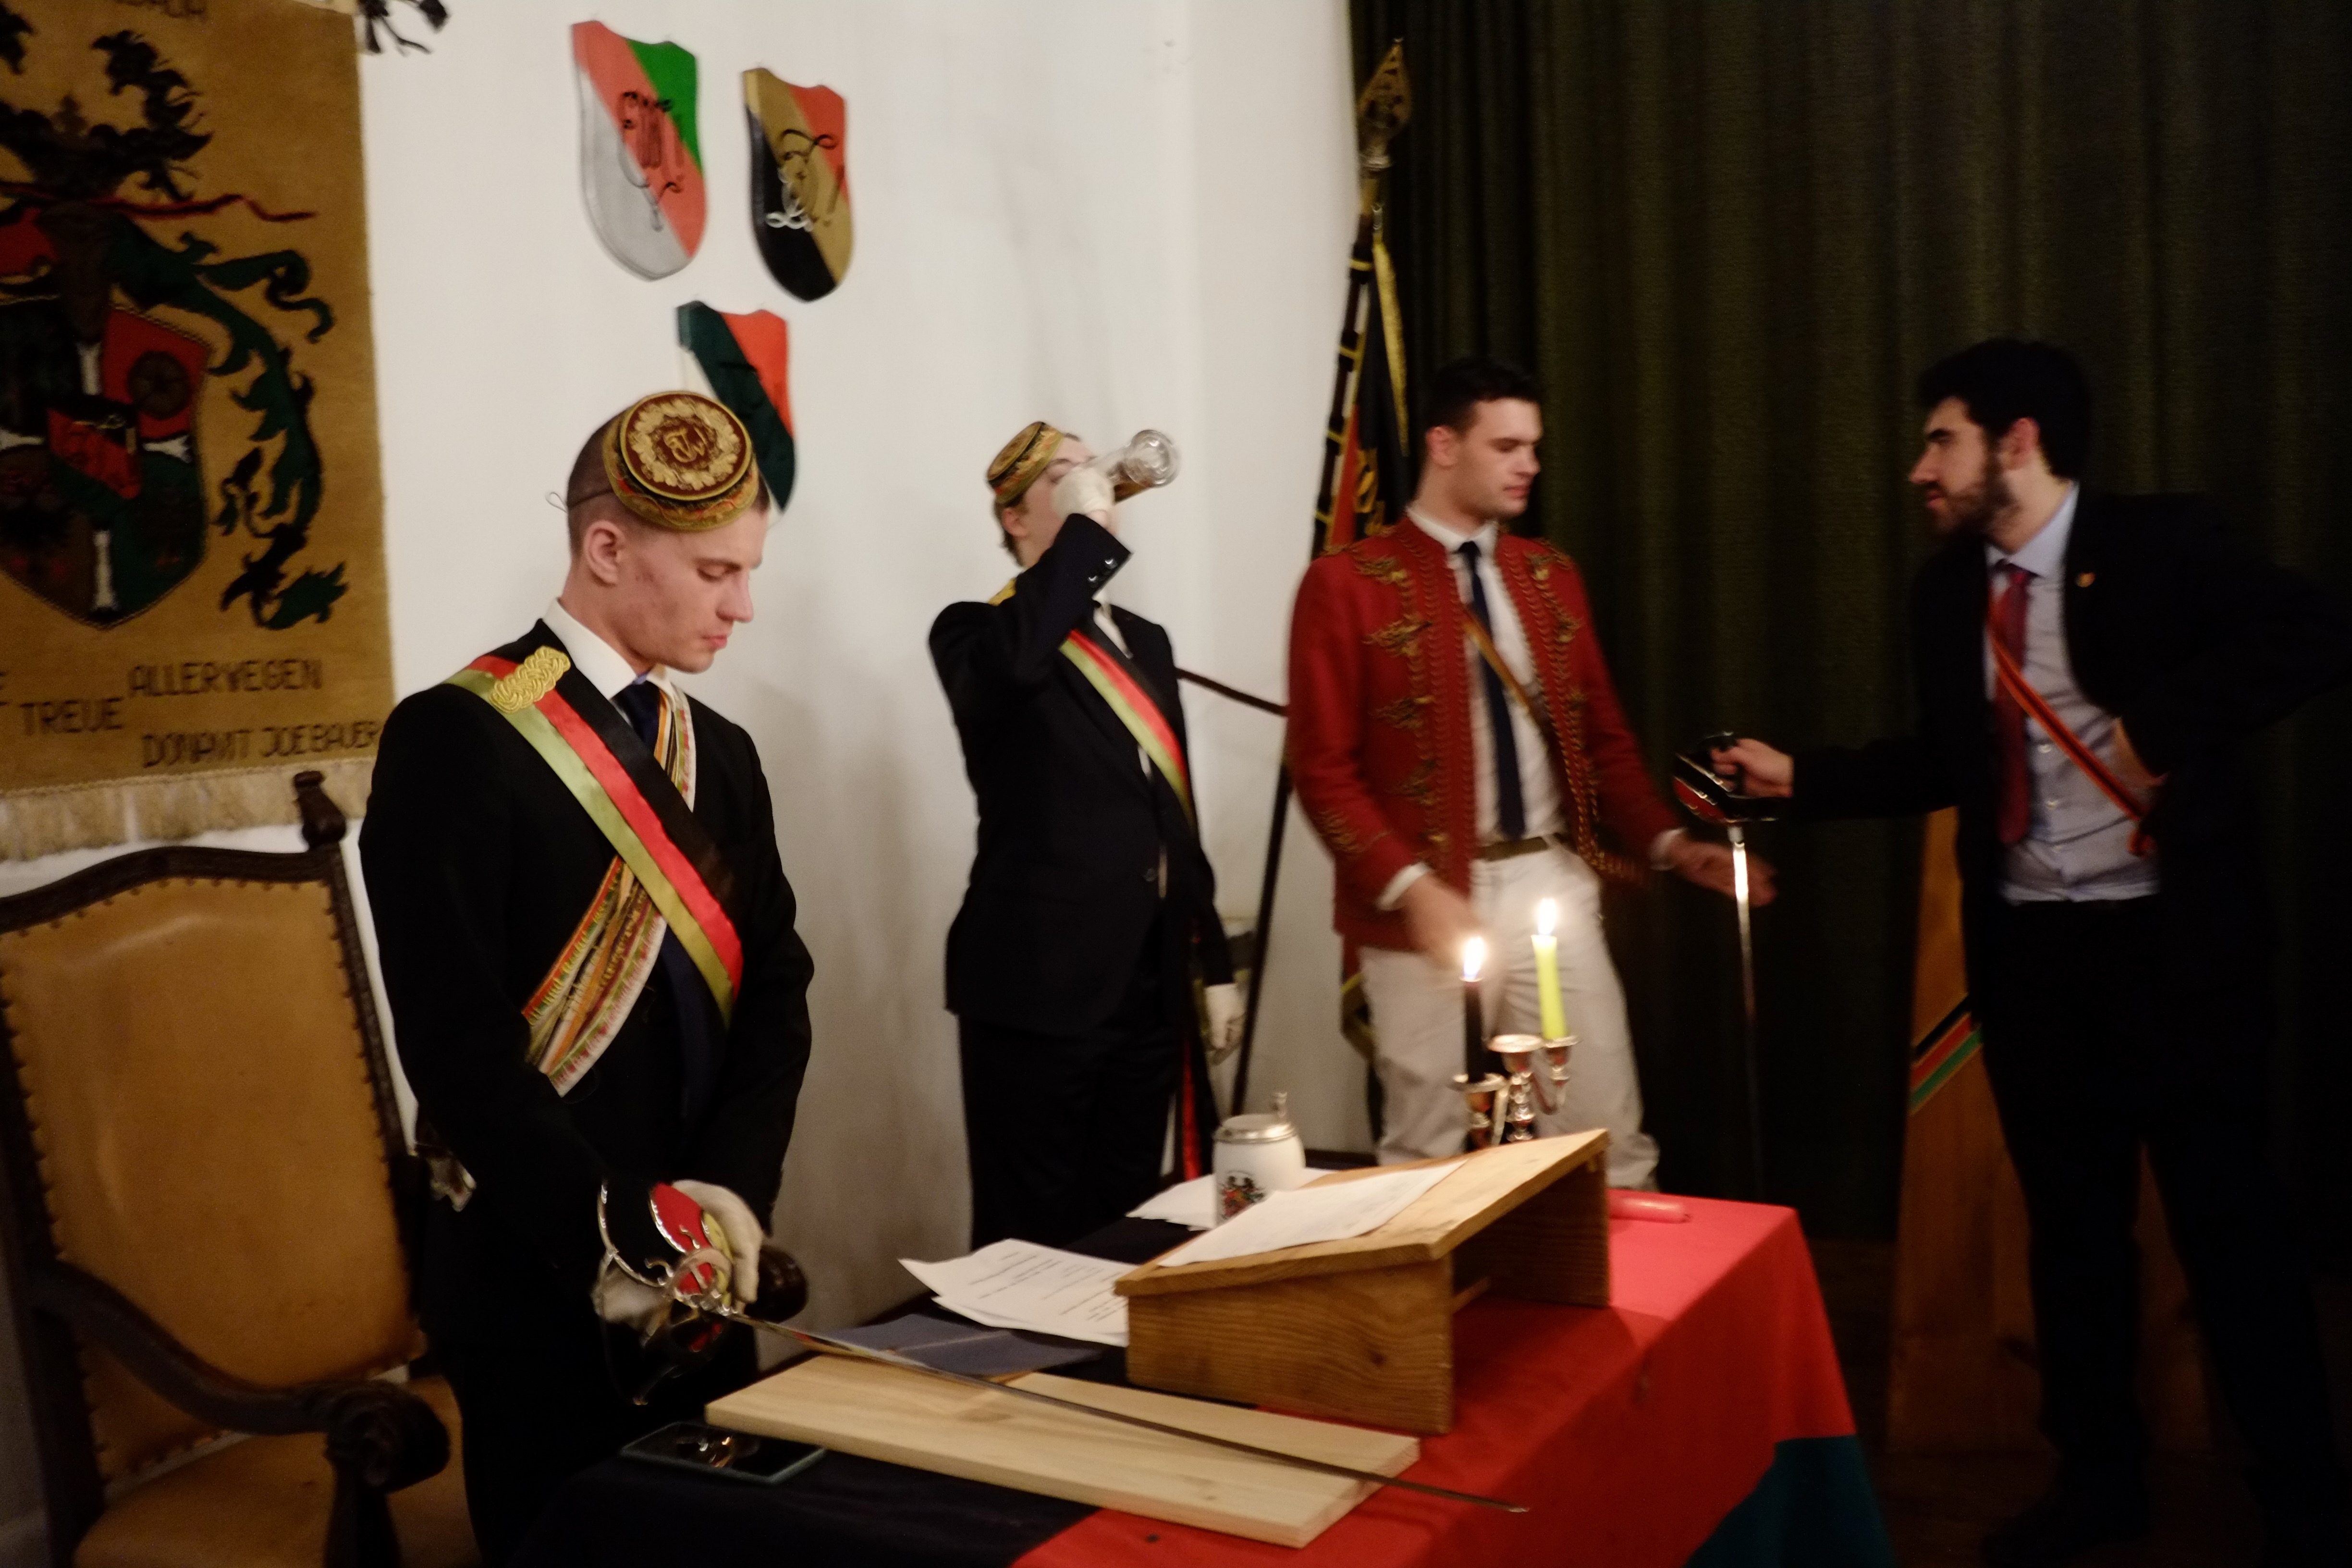
\includegraphics[width=.8\linewidth]{./Bilder/Oelympische Spiele/DSCF6082.jpeg} 
		\caption{Bei der Abkneipe des WS 2023/24\\Von links nach rechts:\\ Senior des SS 2024 Benjamin Buhl \\Fuxmajor Antoine Leyder\\Leiter der Oelympischen Spiele Fabian Heinrich, \\Fux Mathias Brezina (ausgetreten)\\
		} 
	\end{center}
\end{figurehere}

%
%\begin{figurehere}
%	\begin{center}
%		\includegraphics[width=.8\linewidth]{Bilder/pios2}
%		\caption{Realer Aufbau} 
%	\end{center}
%\end{figurehere}